\documentclass[aspectratio=169]{beamer}

% --- PACKAGES ---
\usepackage[utf8]{inputenc}
\usepackage{graphicx}
\usepackage{amsmath}
\usepackage{booktabs}
\usepackage{hyperref}

% --- OVERLEAF DEFAULT BEAMER THEME CONFIGURATION ---
\usetheme{Madrid}
\usecolortheme{default}

% Optional customization popular in Overleaf templates
\usefonttheme{professionalfonts}
\setbeamertemplate{navigation symbols}{} % Remove navigation symbols

% --- PRESENTATION METADATA ---
\title[Ephys \& Passive Electronics]{Ephys, Behavior, \& Passive Electronics}
\subtitle{Day 1.0: Introduction to Neural Recordings \& Passive Circuits}
\author[TENSS 2026]{Antonin Blot}
\institute[TENSS]{Transylvanian Experimental Neuroscience Summer School}
\date[June 2026]{TENSS 2026}

\begin{document}

% ==================== TITLE SLIDE ====================
\begin{frame}
    \titlepage
\end{frame}

% ==================== TABLE OF CONTENTS ====================
\begin{frame}{Outline}
    \tableofcontents
\end{frame}

\section{Overview}

% ==================== SLIDE 2 ====================
\begin{frame}{Module Learning Goals}
    \begin{columns}[T]
        \begin{column}{0.6\textwidth}
            \begin{itemize}
                \item \textbf{Bioelectrical Principles:} How extracellular potentials arise from ionic motion.
                \item \textbf{Recording Chain:} How we sense, amplify, filter, and digitize signals.
                \item \textbf{Passive Electronics 101:} Breadboarding and analyzing components (resistors, dividers, capacitors, filters).
                \item \textbf{Source Impedance:} Understanding how measurement devices affect biological recordings.
                \item \textbf{Closed-Loop Systems:} Combining electrical measurements with behavioral monitoring.
            \end{itemize}
        \end{column}
        \begin{column}{0.35\textwidth}
            \centering
            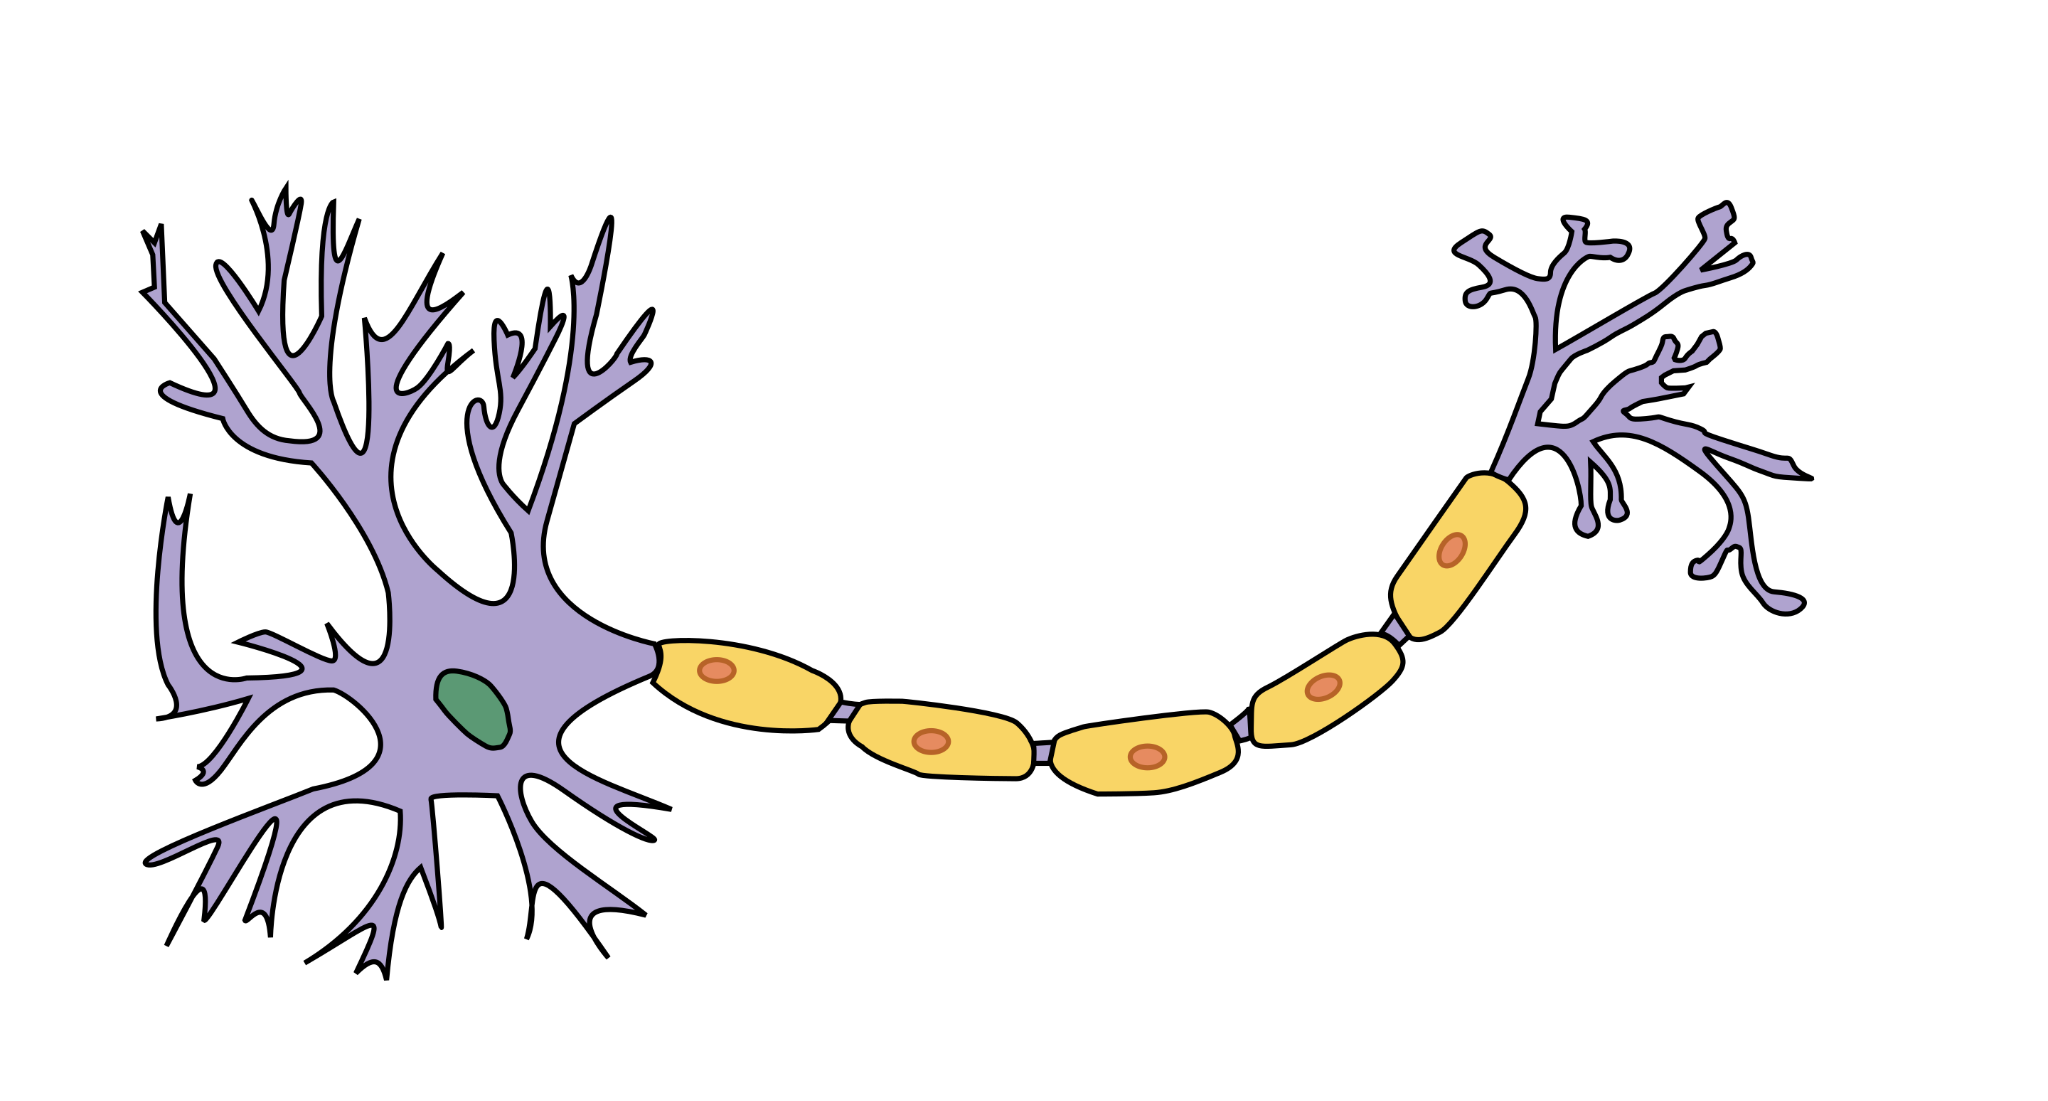
\includegraphics[width=\textwidth]{../docs/media/image1.png}
            \vskip 0.2cm
            {\tiny\color{gray} Neuron/Electrode Interface}
        \end{column}
    \end{columns}
\end{frame}

% ==================== SLIDE 3 ====================
\begin{frame}{Bioelectric Signals in Action}
    \begin{columns}[T]
        \begin{column}{0.55\textwidth}
            \begin{itemize}
                \item \textbf{ECG / EMG:} Massive electrical signals from muscle contractions or cardiac muscle fibers.
                \item \textbf{EEG:} Synaptic potentials summed across millions of cortical neurons, recorded at the scalp.
                \item \textbf{LFP (Local Field Potential):} Intracranial recording showing local synaptic population currents.
                \item \textbf{Single Spikes (Units):} Ultra-fast voltage changes ($<1\text{ ms}$) from individual action potentials.
            \end{itemize}
        \end{column}
        \begin{column}{0.4\textwidth}
            \centering
            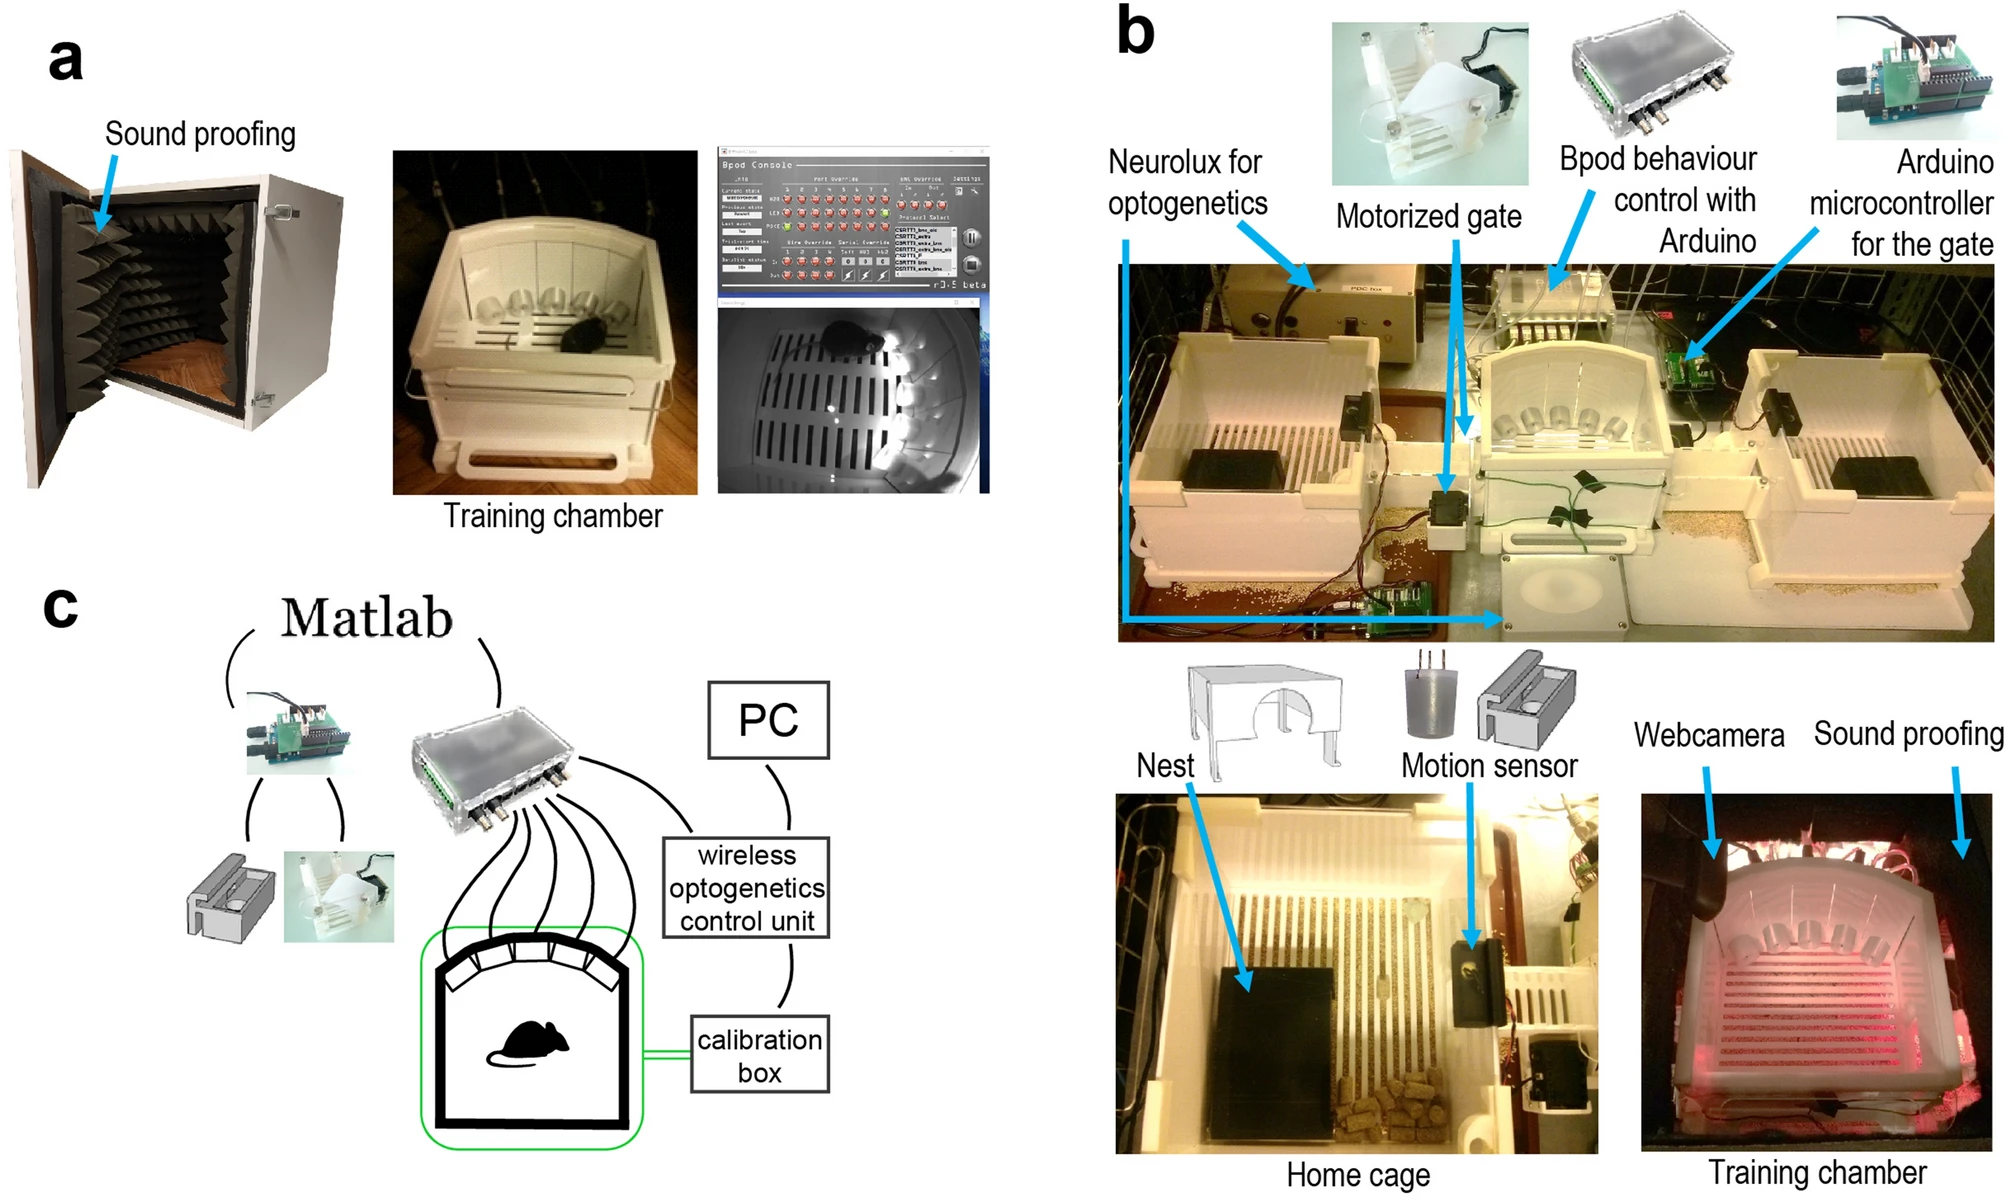
\includegraphics[height=2.2cm]{../docs/media/image20.png}
            \vskip 0.1cm
            {\tiny\color{gray} ECG/EMG Waveforms}
            \vskip 0.2cm
            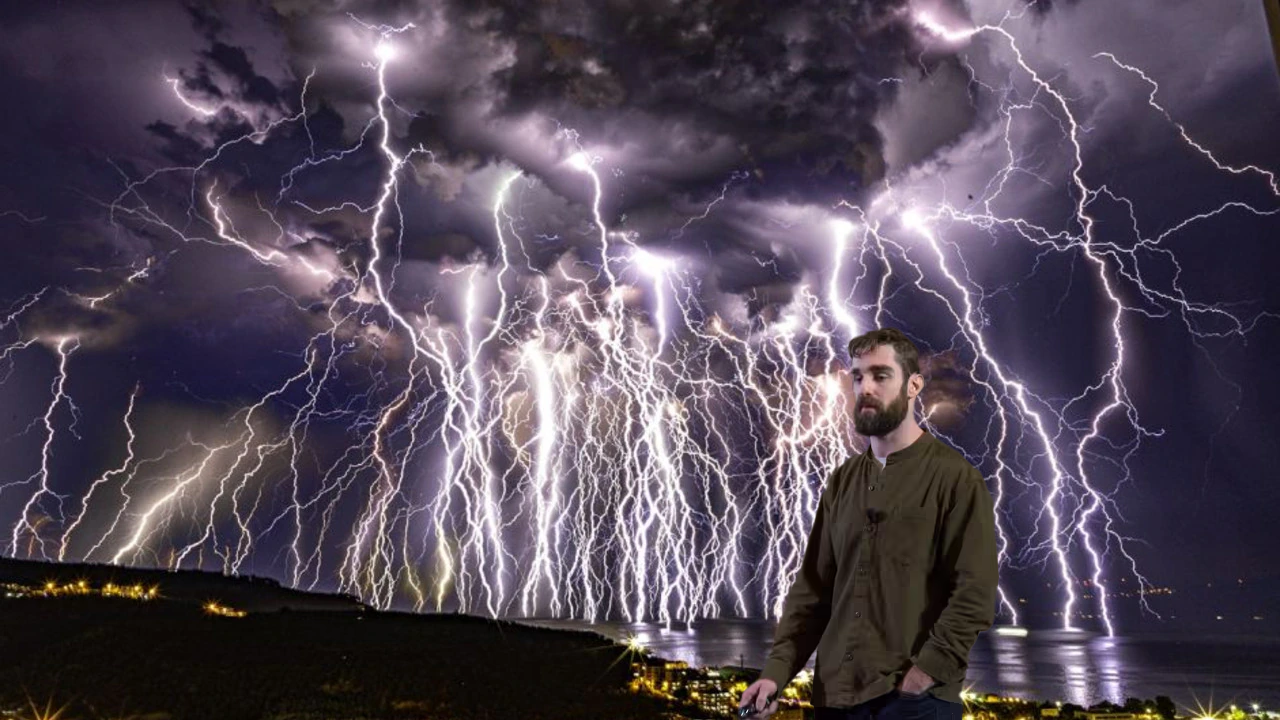
\includegraphics[height=2.2cm]{../docs/media/image16.png}
            \vskip 0.1cm
            {\tiny\color{gray} LFP / Extracellular Spikes}
        \end{column}
    \end{columns}
\end{frame}

% ==================== SLIDE 4 ====================
\begin{frame}{The Recording Chain: ``From Resistor to Spike''}
    \begin{columns}[T]
        \begin{column}{0.6\textwidth}
            \begin{itemize}
                \item \textbf{Electrode Interface:} Picks up ionic current flow and converts it to electronic current.
                \item \textbf{Amplifier (Active):} Scales tiny extracellular microvolts ($\mu\text{V}$) to voltages readable by digitizers.
                \item \textbf{Filters (Passive/Active):} Eliminates noise and separates slow LFPs from fast spikes.
                \item \textbf{Digitizer (ADC):} Samples the continuous analog voltage into binary arrays for computer storage.
            \end{itemize}
        \end{column}
        \begin{column}{0.35\textwidth}
            \centering
            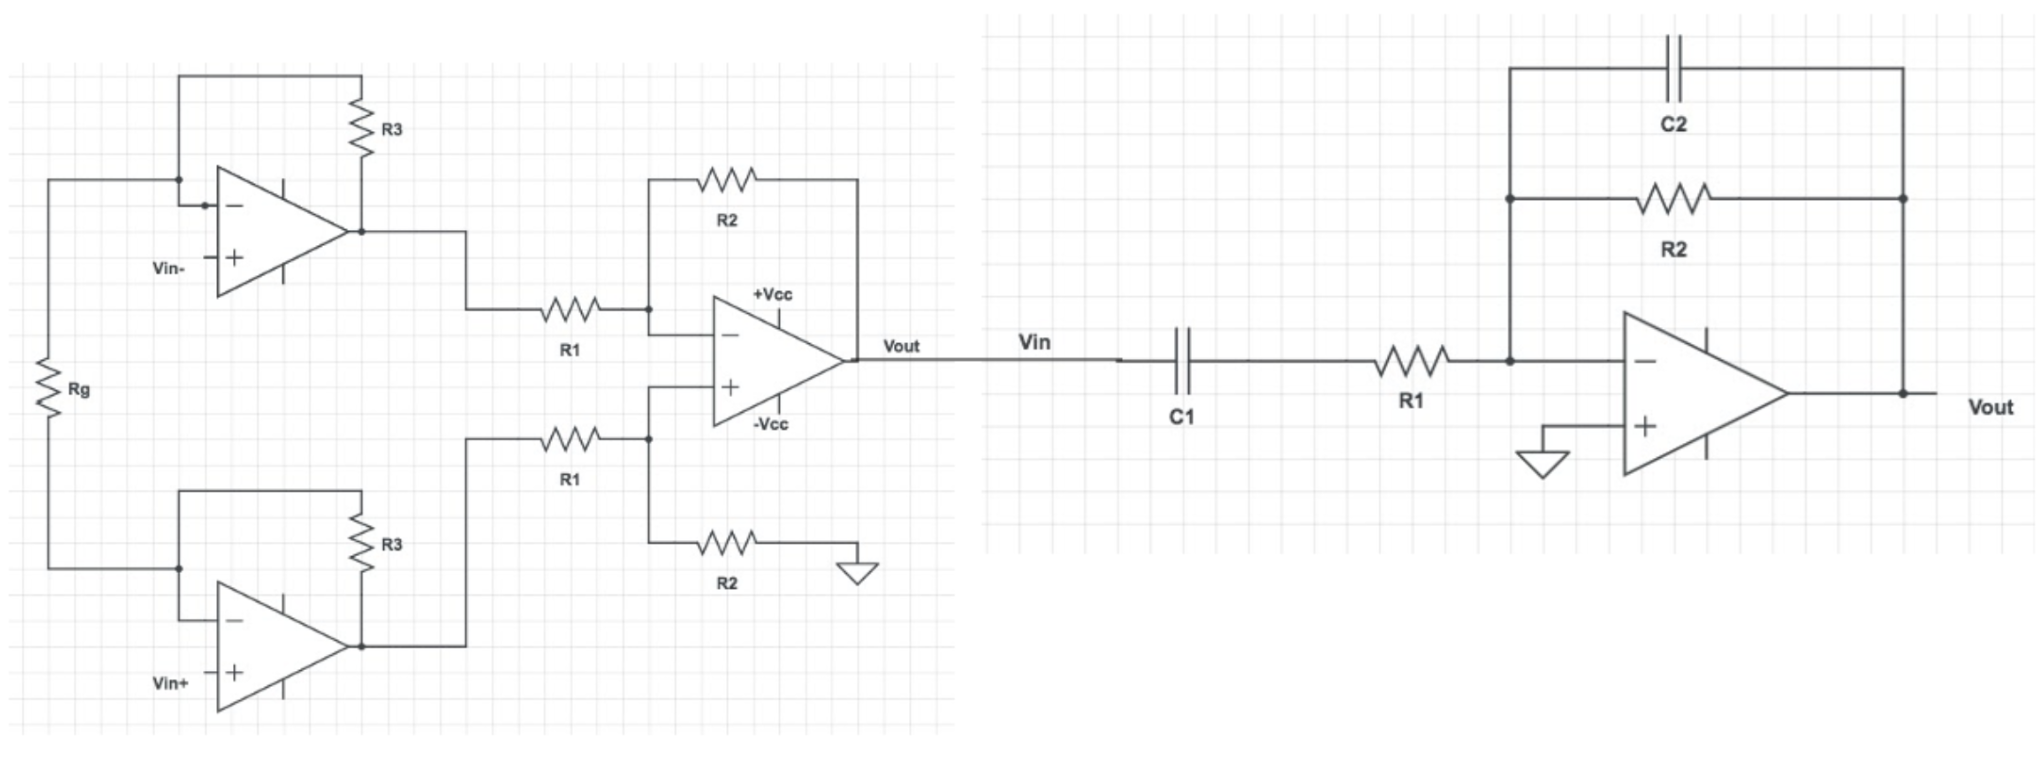
\includegraphics[width=\textwidth]{../docs/media/image9.png}
            \vskip 0.2cm
            {\tiny\color{gray} Signal Recording Flow}
        \end{column}
    \end{columns}
\end{frame}

% ==================== SLIDE 5 ====================
\begin{frame}{Behavior and Closed-Loop Systems}
    \begin{columns}[T]
        \begin{column}{0.6\textwidth}
            \begin{itemize}
                \item \textbf{Closed-loop logic:} Reading sensor inputs (e.g., beam-breaks) to drive actuators (e.g., LED cues, optogenetic lasers).
                \item \textbf{Open Ephys Integration:} Routing behavioral cues and ephys signals into a synchronized acquisition stream.
                \item \textbf{Real Life is Messy:} Noise, parasitic capacitance, and ground loops require solid ground isolation.
            \end{itemize}
        \end{column}
        \begin{column}{0.35\textwidth}
            \centering
            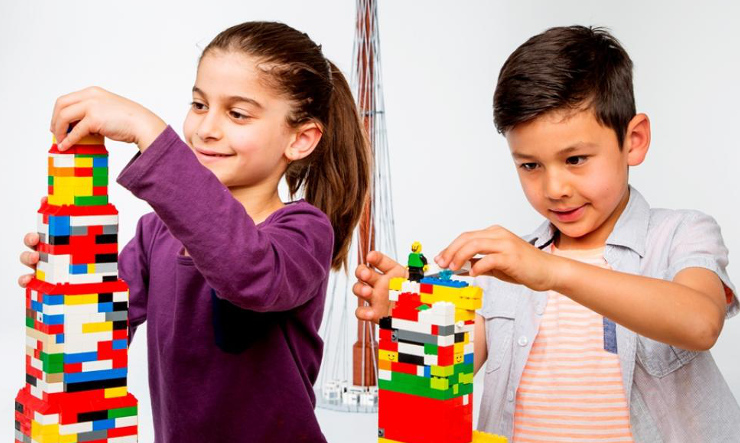
\includegraphics[width=\textwidth]{../docs/media/image7.png}
            \vskip 0.2cm
            {\tiny\color{gray} Lego Behavioral Arena}
        \end{column}
    \end{columns}
\end{frame}

\section{Physics}

% ==================== SLIDE 6 ====================
\begin{frame}{Charged Particles \& Electric Fields}
    \begin{columns}[T]
        \begin{column}{0.6\textwidth}
            \begin{itemize}
                \item \textbf{Biological Charges:} Our charge carriers are ions ($\text{Na}^+, \text{K}^+, \text{Cl}^-, \text{Ca}^{2+}$).
                \item \textbf{Coulomb Force:} Like charges repel, opposite charges attract.
                \item \textbf{Electric Field ($\vec{E}$):} Space vector describing the force a unit charge would feel.
                \item \textbf{Charge Motion:} An electric potential (voltage) difference creates an electric field, exerting a force:
                \begin{equation*}
                    \vec{F} = q \cdot \vec{E}
                \end{equation*}
                This force pushes the ions, generating biological currents.
            \end{itemize}
        \end{column}
        \begin{column}{0.35\textwidth}
            \centering
            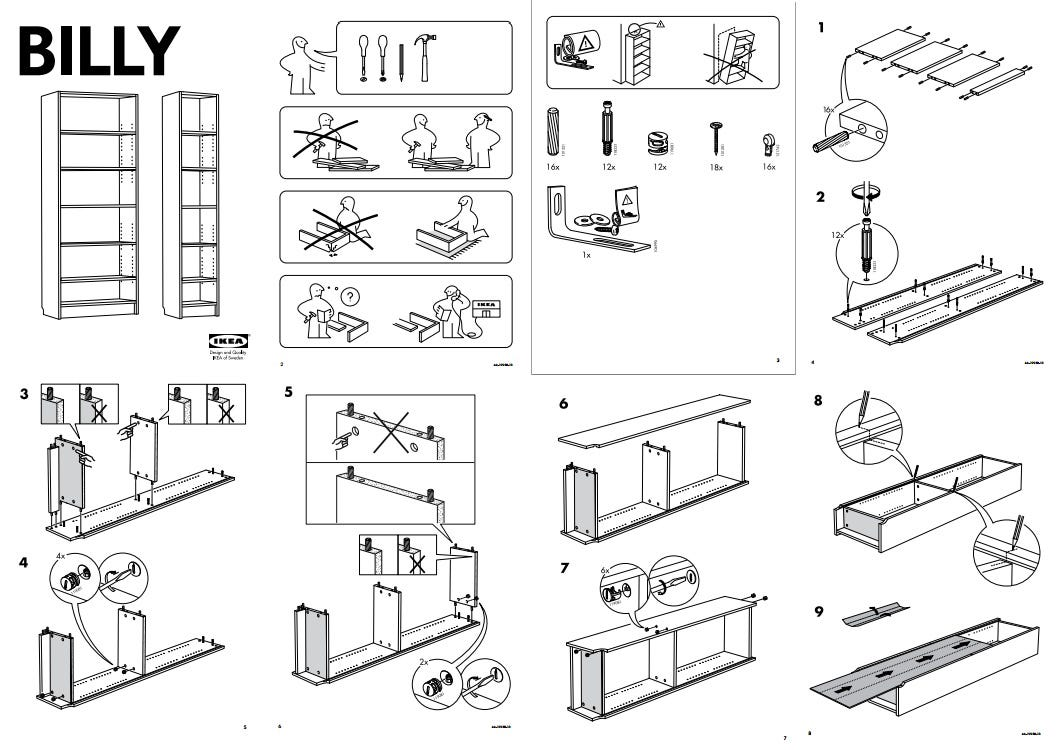
\includegraphics[width=\textwidth]{../docs/media/image21.png}
            \vskip 0.2cm
            {\tiny\color{gray} Electric Field Vector Map}
        \end{column}
    \end{columns}
\end{frame}

\section{Circuits}

% ==================== SLIDE 7 ====================
\begin{frame}{Voltage, Current, \& Resistance}
    \begin{columns}[T]
        \begin{column}{0.6\textwidth}
            \begin{itemize}
                \item \textbf{Voltage ($V$):} The potential energy difference pushing charge between two points. Measured in Volts ($V$).
                \item \textbf{Current ($I$):} The flow rate of charges through a conductor. Measured in Amperes ($A$).
                \item \textbf{Resistance ($R$):} Opposition to charge movement. Impedes current and dissipates energy as heat. Measured in Ohms ($\Omega$).
            \end{itemize}
            \begin{block}{Ohm's Law}
                \large
                \begin{equation*}
                    V = I \cdot R
                \end{equation*}
            \end{block}
        \end{column}
        \begin{column}{0.35\textwidth}
            \centering
            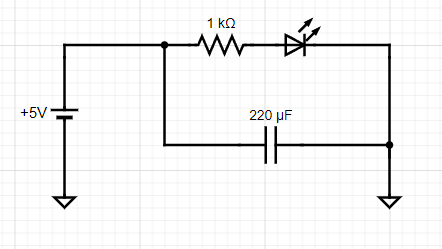
\includegraphics[width=\textwidth]{../docs/media/image33.png}
            \vskip 0.2cm
            {\tiny\color{gray} Current Flow Concept}
        \end{column}
    \end{columns}
\end{frame}

% ==================== SLIDE 8 ====================
\begin{frame}{Hydraulic Analogy}
    \centering
    \begin{tabular}{lll}
        \toprule
        \textbf{Electrical Concept} & \textbf{Hydraulic Counterpart} & \textbf{Physical Action} \\
        \midrule
        \textbf{Voltage ($V$)} & Water Pressure & The force pushing charge/water. \\
        \textbf{Current ($I$)} & Flow Rate (Liters/Sec) & The volume of charge/water in motion. \\
        \textbf{Resistance ($R$)} & Pipe Restriction / Narrowing & Limits the flow rate for a given pressure. \\
        \textbf{Ground ($0\text{V}$)} & Sea Level & The arbitrary reference potential height. \\
        \bottomrule
    \end{tabular}
    \vspace{0.4cm}
    \begin{block}{Note}
        Just like water needs a height/pressure gradient to flow, electrical charges require a voltage difference to flow. No gradient means no current.
    \end{block}
\end{frame}

% ==================== SLIDE 9 ====================
\begin{frame}{Conservation of Charge \& Loops}
    \begin{columns}[T]
        \begin{column}{0.6\textwidth}
            \begin{itemize}
                \item \textbf{Loop Topology:} Because charge is conserved, current cannot pile up anywhere. It must travel in closed loops.
                \item \textbf{Ground Reference:} Voltage is always relative. Ground ($0\text{V}$) is an arbitrarily selected common pathway to measure other potentials against.
                \item \textbf{Kirchhoff's Current Law:} The sum of currents entering any junction (node) must equal the sum of currents leaving it:
                \begin{equation*}
                    \sum I_{\text{in}} = \sum I_{\text{out}}
                \end{equation*}
            \end{itemize}
        \end{column}
        \begin{column}{0.35\textwidth}
            \centering
            \includegraphics[width=\textwidth]{../docs/media/image46.png}
            \vskip 0.2cm
            {\tiny\color{gray} Loop Schematic}
        \end{column}
    \end{columns}
\end{frame}

% ==================== SLIDE 10 ====================
\begin{frame}{Series \& Parallel Resistances}
    \begin{columns}[T]
        \begin{column}{0.55\textwidth}
            \textbf{Series Resistors}
            \begin{itemize}
                \item Current is identical through all resistors.
                \item Overall resistance increases.
                \item \begin{equation*} R_{\text{total}} = R_1 + R_2 + \dots \end{equation*}
            \end{itemize}
            \vspace{0.1cm}
            \textbf{Parallel Resistors}
            \begin{itemize}
                \item Voltage drop is identical across all resistors.
                \item Total resistance drops.
                \item \begin{equation*} \frac{1}{R_{\text{total}}} = \frac{1}{R_1} + \frac{1}{R_2} + \dots \end{equation*}
            \end{itemize}
        \end{column}
        \begin{column}{0.4\textwidth}
            \centering
            \includegraphics[width=0.85\textwidth]{../docs/media/image67.png}
            \vskip 0.2cm
            {\tiny\color{gray} Resistors in Series and Parallel}
        \end{column}
    \end{columns}
\end{frame}

% ==================== SLIDE 11 ====================
\begin{frame}{The Voltage Divider}
    \begin{columns}[T]
        \begin{column}{0.6\textwidth}
            \begin{itemize}
                \item \textbf{Function:} Attenuates/splits an input voltage using resistors.
                \item \textbf{Passive Attenuation:} Because this is passive, $V_{\text{out}}$ can never exceed $V_{\text{in}}$ (gain is always $\le 1$).
            \end{itemize}
            \begin{block}{Formula}
                The output voltage is a fraction of the input:
                \begin{equation*}
                    V_{\text{out}} = V_{\text{in}} \cdot \frac{R_2}{R_1 + R_2}
                \end{equation*}
            \end{block}
        \end{column}
        \begin{column}{0.35\textwidth}
            \centering
            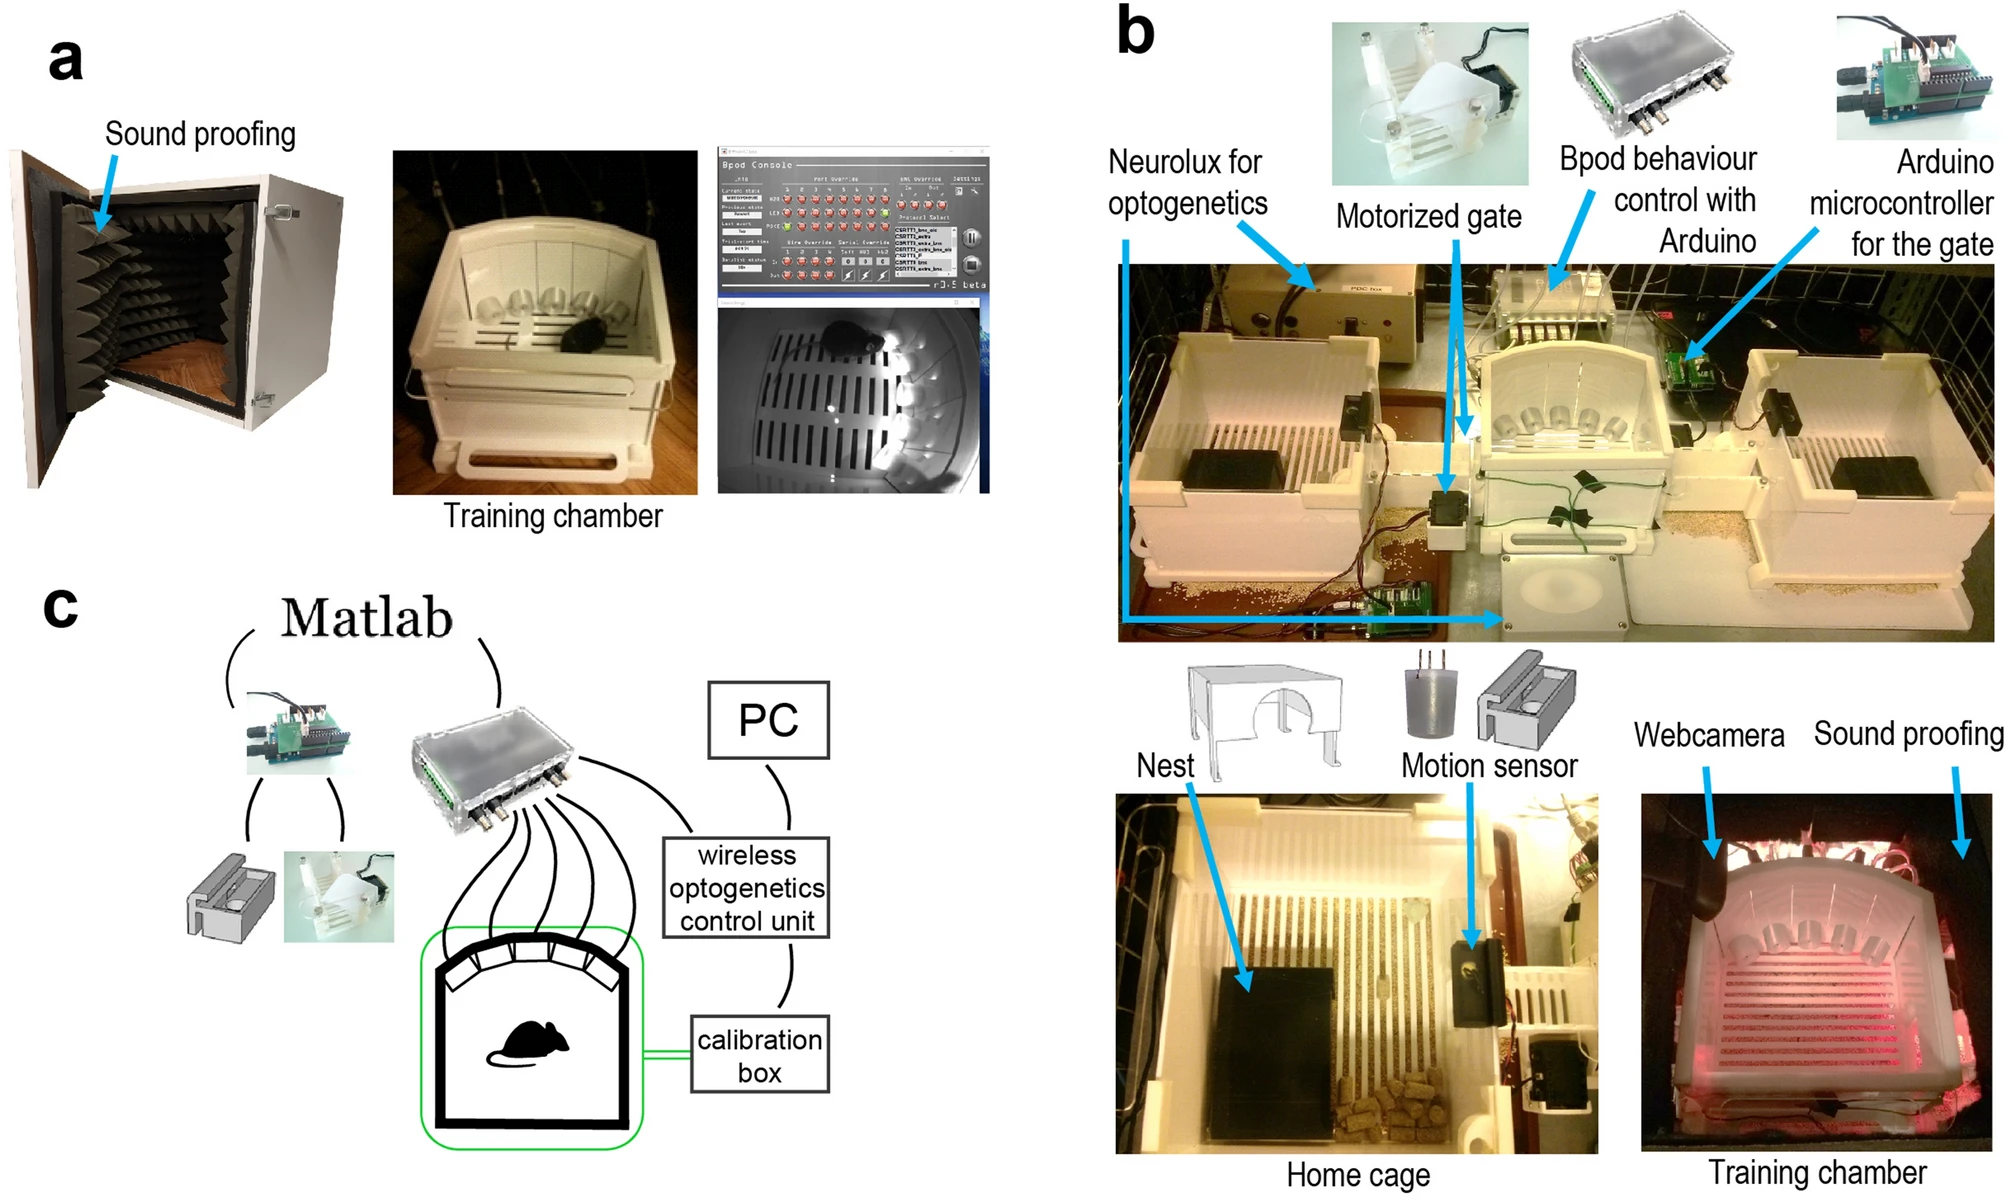
\includegraphics[width=\textwidth]{../docs/media/image20.png}
            \vskip 0.2cm
            {\tiny\color{gray} Voltage Divider Circuit (Exercise 1-1)}
        \end{column}
    \end{columns}
\end{frame}

% ==================== SLIDE 12 ====================
\begin{frame}{Source Impedance \& Loading}
    \begin{columns}[T]
        \begin{column}{0.6\textwidth}
            \begin{itemize}
                \item \textbf{The Problem:} Biological electrodes have a series resistance ($R_s$). Recording devices have a shunt resistance to ground ($R_{\text{sh}}$).
                \item \textbf{Divider Effect:} These form an unintended voltage divider:
                \begin{equation*}
                    V_{\text{measured}} = V_{\text{bio}} \cdot \frac{R_{\text{sh}}}{R_s + R_{\text{sh}}}
                \end{equation*}
                \item \textbf{Loading:} If $R_{\text{sh}}$ is low (e.g. $220\,\Omega$), the measured signal drops close to $0$.
                \item \textbf{Rule of thumb:} Ensure recording input impedance is massive: $R_{\text{sh}} \gg R_s$.
            \end{itemize}
        \end{column}
        \begin{column}{0.35\textwidth}
            \centering
            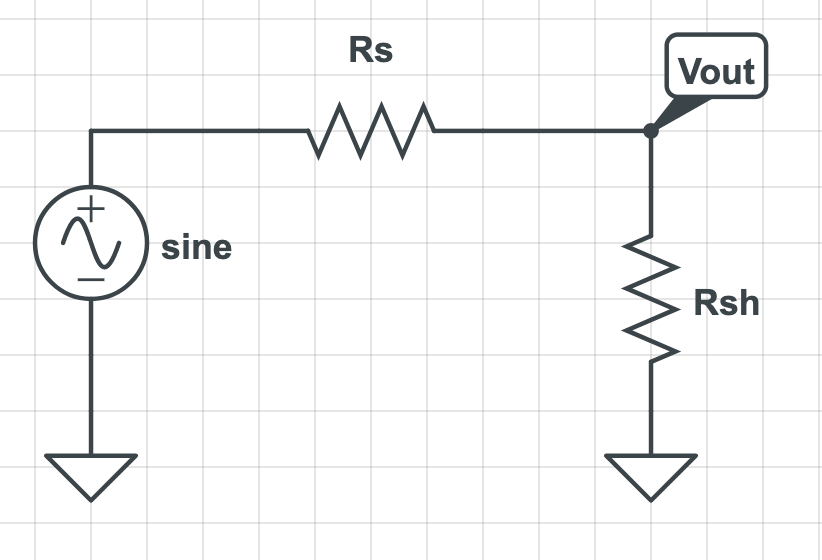
\includegraphics[width=\textwidth]{../docs/media/image23.png}
            \vskip 0.2cm
            {\tiny\color{gray} Impedance Loading Model (Exercise 1-3)}
        \end{column}
    \end{columns}
\end{frame}

\section{Filters}

% ==================== SLIDE 13 ====================
\begin{frame}{Capacitors \& Charge Storage}
    \begin{columns}[T]
        \begin{column}{0.6\textwidth}
            \begin{itemize}
                \item \textbf{Definition:} Two conductors separated by an insulator that store charge ($Q = C \cdot V$).
                \item \textbf{Biology:} The lipid cell membrane acts as a capacitor, storing charge and delaying potential changes.
            \end{itemize}
            \begin{block}{Dynamic Behavior}
                Capacitors oppose sudden changes in voltage. Current is proportional to rate of change:
                \begin{equation*}
                    I = C \cdot \frac{dV}{dt}
                \end{equation*}
            \end{block}
        \end{column}
        \begin{column}{0.35\textwidth}
            \centering
            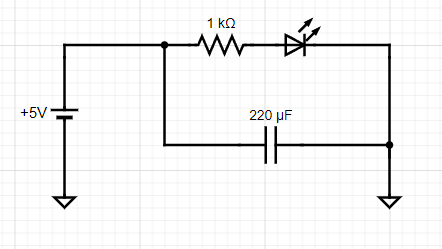
\includegraphics[width=\textwidth]{../docs/media/image33.png}
            \vskip 0.2cm
            {\tiny\color{gray} Capacitor Circuit (Exercise 1-4)}
        \end{column}
    \end{columns}
\end{frame}

% ==================== SLIDE 14 ====================
\begin{frame}{Capacitive Reactance}
    \begin{columns}[T]
        \begin{column}{0.6\textwidth}
            \begin{itemize}
                \item \textbf{Frequency-Dependent Resistance:} To AC signals, a capacitor acts like a resistor whose value (reactance $X_c$) changes with frequency:
                \begin{equation*}
                    X_c = \frac{1}{2\pi f C}
                \end{equation*}
                \item \textbf{DC ($f = 0\,\text{Hz}$):} $X_c = \infty$. Capacitors block DC voltages completely.
                \item \textbf{AC ($f \rightarrow \infty$):} $X_c \rightarrow 0$. High frequencies pass freely.
            \end{itemize}
        \end{column}
        \begin{column}{0.35\textwidth}
            \centering
            \vspace{1cm}
            \begin{block}{AC vs. DC Flow}
                \centering
                \textbf{DC Input} $\rightarrow$ Blocked \\
                \vspace{0.2cm}
                \textbf{AC Input} $\rightarrow$ Passed
            \end{block}
        \end{column}
    \end{columns}
\end{frame}

% ==================== SLIDE 15 ====================
\begin{frame}{Passive RC Filters}
    \begin{columns}[T]
        \begin{column}{0.6\textwidth}
            \begin{itemize}
                \item \textbf{High-Pass Filter:} Capacitor in series, resistor to ground. Passes high frequency spikes, blocks DC drift.
                \item \textbf{Low-Pass Filter:} Resistor in series, capacitor to ground. Shunts high frequencies to ground, leaving slow LFPs.
            \end{itemize}
            \begin{block}{Cutoff Frequency ($f_c$)}
                Frequency where output amplitude is reduced by $\sim$30\%:
                \begin{equation*}
                    f_c = \frac{1}{2\pi R C}
                \end{equation*}
            \end{block}
        \end{column}
        \begin{column}{0.35\textwidth}
            \centering
            
\includegraphics[width=\textwidth]{../docs/media/image10.png}
            \vskip 0.2cm
            {\tiny\color{gray} RC Filter Circuits (Part 2)}
        \end{column}
    \end{columns}
\end{frame}

% ==================== SLIDE 16 ====================
\begin{frame}{Summary \& Prep}
    \begin{itemize}
        \item \textbf{Voltage Dividers} govern scaling and electrode loading. Remember: keep amplifier input impedance high!
        \item \textbf{Capacitors} behave dynamically: they block slow drift (DC) and pass fast signals (AC).
        \item \textbf{RC Circuits} let you construct simple high-pass and low-pass filters to isolate target signals.
    \end{itemize}
    \vspace{0.4cm}
    \begin{block}{Ready for Part 1}
        You will now build a physical voltage divider, measure biological source loading, and capture capacitor discharge curves on the oscilloscope.
    \end{block}
\end{frame}

\end{document}
